\documentclass[a4paper, 11pt]{scrartcl}

% font, language
%\usepackage[utf8]{inputenc}
%\usepackage[T1]{fontenc}
%\usepackage{lmodern}

\usepackage{todonotes}

\usepackage{fontspec}
\setmainfont{Latin Modern Roman}

\usepackage{polyglossia}
%\setmainlanguage[babelshorthands=true]{german}
\setmainlanguage{english}

% \usepackage[ngerman]{babel}
\usepackage[autostyle]{csquotes}

% graphics
\usepackage{graphicx}
\graphicspath{ {images/} }

% code highlighting
\usepackage{listings}
\usepackage{color}
\lstset{ % General setup for the package
	language=java
}

% toc depth
\setcounter{tocdepth}{4}
\setcounter{secnumdepth}{4}

% bib
\usepackage[backend=biber]{biblatex}
\addbibresource{references.bib}
\usepackage{hyperref}
\usepackage{xcolor}
\hypersetup{
	colorlinks,
	linkcolor={red!0!black},
	citecolor={blue!70!black},
	urlcolor={blue!70!black}
}

\usepackage{enumitem}
\setlist[enumerate]{label*=\arabic*.}

% title, author
\title{Exposè zur Bachelor-Thesis}
\author{Roman Quistler}

\begin{document}
	
	\begin{titlepage}
	\centering
	
\includegraphics[width=0.30\textwidth]{hsb_logo.png}
	\par\vspace{1cm}
	{\scshape\LARGE Hochschule Bremen \par}
	\vspace{1cm}
	{\scshape\Large Bachelorarbeit  \par}
	\vspace{1.5cm}
	{\LARGE\bfseries Entwicklung eines Model-View-Intent Framework für die Plattform Android\par}
	\vspace{0.5cm}
	{\normalsize\itshape Medieninformatik B.Sc. \par}
	\vspace{2cm}
	{\Large\itshape Roman Quistler \par}
	\vfill
	\vfill
	{\large\today\par}
\end{titlepage}
	
	\pagenumbering{gobble}
	\newpage
	\tableofcontents
	\newpage
	\pagenumbering{arabic}
	
	\section{Introduction}
\label{sec:introduction-words}
	
Das Entwickeln von Applikationen ist nicht einfach.
	
	\section{Problem and solution}
	\label{sec:problem-solution}
	
	\subsection{Problem}
\label{subsec:problem}

Today's applications seem to be increasing in complexity over the last few years. 
Especially in the field of frontend development, the range of functions has increased \cite{kevin2018}.
The web development has transitioned from server rendered, page-reloading websites, to modern so called single page applications or SPA's.
The user 

But the same applies to the mobile world. Social networks, navigation, sharing and editing files together.
The functionality that a application includes today

More functionality does thus in some sense translate into more conditions the application can be in. 

Considering a simple login screen feature inside an android application. A user can provide authentication credentials
in order to login. It's possible that a user enters wrong credentials, which in turn can be handled by the app by displaying
a short description of what went wrong, like an error message.
If the user then provides the wrong credentials more than three times, his user account could get locked. 
This also in some way must be expressed by the application.
He could also make use of the "Forgot Password" functionality. That could allow the user to navigate away from the application
into a browser window instead in order to reset the password.

% fixme{correct tables for finite statemachine}
% State Transition Table
| State/Event | Logging in | Logging out |
| Logged in | x | x |
| Logged out | x | x |

Immediately it becomes clear that there are already four possible states in which the application can be in.
A developer thus ends up with states * events possible states which must be considered and handled appropriately.

For example the application might be in the state of "logging in" and then a user tries to transition into
the event of "logging in" again, which might not be desirable.
 
The complexity for such a "simple" or at least standard feature grows linearly with the amount
of states and events that are introduced into the application.

With the increasing states and events it becomes harder and harder to have a general overview of all
possible states.

Given that a project grows and more and more functionality is added to the codebase, the more 
important the state becomes and the harder it becomes to introduce state as an afterthought.

In most cases \ref{unreferenced statement/claim}, an application communicates with other interfaces, such as a back-end or local database.
On mobile devices it's also often necessary to know the GPS status, whether mobile data is enabled or not, etc. 

A click of a user thus can cause many changes inside and outside of the application.
A developer must be aware of all the possible outcomes, react to them and save what has happened.

By increased application complexity the necessity to make sure the application behaves exactly
as expected in all cases increases. This property in software development is referred to a deterministic system, 
which states \ref{wiki-deterministic} that a deterministic model always produce the same output from a given starting
condition or initial state. This is a desirable property because it makes it simpler to predict and reason about events and states
in which the application can be within.

The problem of opposite, nondeterministic software is thus that it makes the code less readable since
it's impractical to gloss over the code to determine the potential output of a function call.

Code readability becomes a vital part in codebases when they start growing in complexity and size. But also 
when they are being worked on by more people than just the person who initially wrote it.

~~productive in writing code instead of deciphering other peoples codes it becomes essential.~~

A product of readability is another important property which is increased maintainability.
Maintainability ties into the notion of not having to rewrite parts of the codebase
that is not directly related to the functionality being added or modified.

The arguably most well known remedy for this problem is the SOLID principle, first
proposed by \ref{Robert C. Martin } in his paper \ref{Design Principles and Design Patterns}
published in the year 2000.

* Single responsibility principle
* Open-closed principle
* Liskov substitution principle
* Interface segregation principle
* Dependency inversion principle


% Problem End -- Summary
Thus far it can be summaries the problem to be that of maintainability, flexibility and readability.
These are basic concepts that unless respected have a domino-like side-effects 

And core to this problem is managing the applications state in a way that it can survive platform
restrictions like for example unexpected process death or in android specifically a configuration change
ie device rotation.

~~Once this basic login feature is implemented another problem emerges which is to add more functionality
like for example a 'protected view' which requires the user to be logged in 
this view should not be reachable from the 'logged out' state without
transition into 'logged in' state first.~~

Side-problems solved by solution to main problem

%* [x] Deterministic
%* [x] Open for extension, closed for modification

%* [x] Maintainability
%    * [x] Code readability

% # Problematic

* Nondeterministic
* Closed for extension, open for modification
* Unreadable code
* Unmaintainable code

%\begin{figure}[h]
%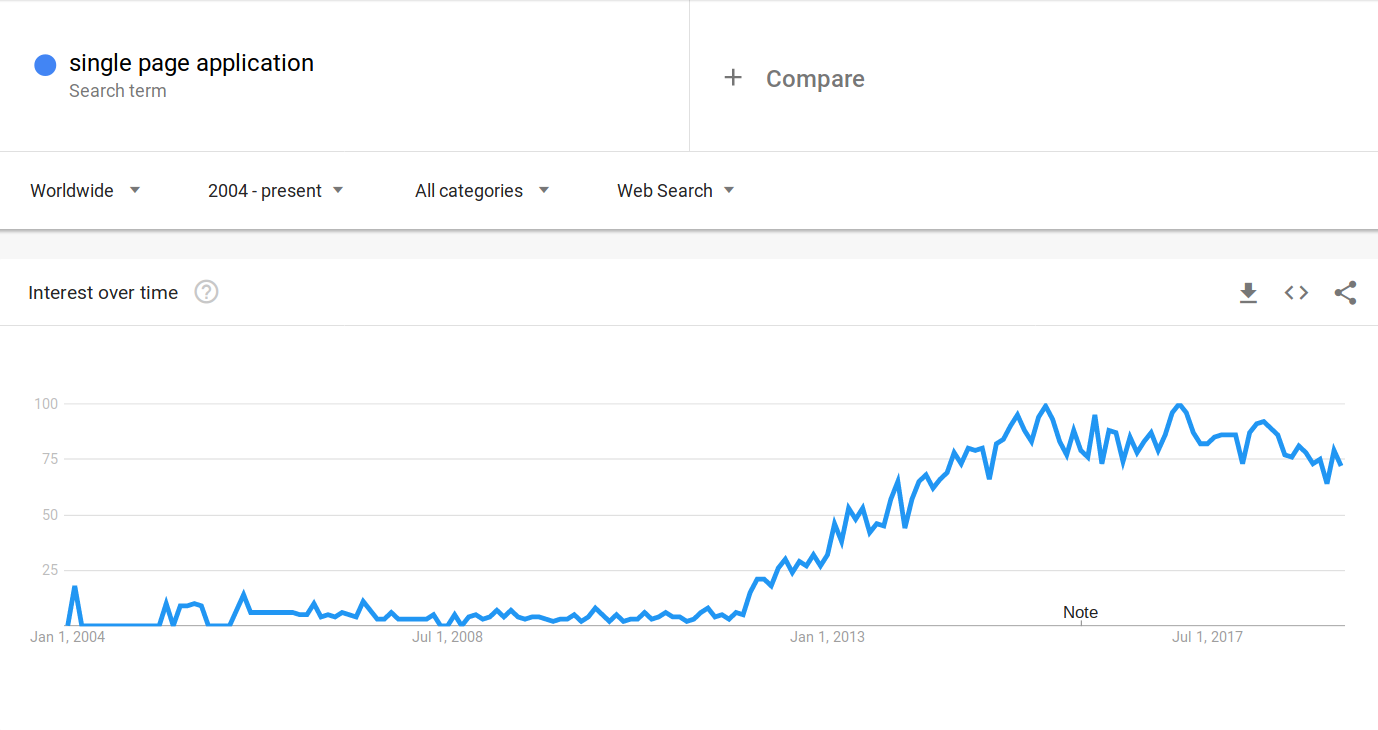
\includegraphics[width=0.97\textwidth]{google-trends-spa}
%\centering
%\caption{Google trends: single page application}
%\label{fig:google-trends-spa}
%\end{figure}

The developer must thus manage the state. The problem is to find a good design pattern, 
which solves the state problem by not treating it as an afterthought. 

\todo{in such a way that it respects SOLID/DRY etc}

\todo{mention reactive programming}

% shared mutable state = bad
% https://www3.nd.edu/~kogge/courses/cse30151-fa17/Public/other/tikz_tutorial.pdf
	
	\subsection{Solution}
\label{subsec:solution}

% - to take a deeper look at MVI
% - where it comes from (flux + redux + mvc)
% - at existing solution
% - what they might do badly
% - solution or goal is to develop a framework


\newpage
In order to overcome the mentioned problem, the aim will be to take a deeper look at what is important to understand and successfully implement MVI.
For this it is essential to get a better overview over archhitectural patterns in general. Before this can be done meaningfully the first step must be 
to analyze why they came to life in the first place and what the exact motivation was. Further the problem they try to solve should be layed out in more detail to 
get the bigger picture. In order to do justice to that, it is a necessity to review the history of architectural patterns and to work out how they have evolved over time.
By doing that it will also be possible to track down the issues that each of this architectural patterns brings with it.
\\
\\
After this is accomplished, the next step is to study the origins of Model-View-Intent. The beginning is made by the JavaScript library React and the application architecture
Flux, which introduced the concept of the unidirectional flow for building user interfaces. It is necessary to clarify which idea is hidden behind it and what it does
better than previous solutions. All components of this framework should be examined and shortly explained. Following on from this, a further improvement(?) of Flux will 
be discussed: Redux. Differences to the idea and terminology of Flux will be pointed out and evaluated.
\\
\\
Since Mode-View-Intent takes some of its inspiration regarding its structure from Mode-View-Cotroller, it is imperative (crucial?) to dedicate a section to it as well.
In this section, the similarities and differences will be identified and illustrated to get a better grasp, as to why it served as a source of inspiration.

	\section{Specific Tasks}
\label{sec:specific-tasks}

The following tasks are necessary for the realization of the Bachelor Thesis:
%
\begin{itemize}
    \item Research: Collection and comparison of further literature, for a deeper understanding of the topic.
    \item Requirement analysis:
        \begin{itemize}
        	\item
        \end{itemize}
    \item Design:
    \item Prototypical implementation: Development of a native Android application, in which the determined requirements are implemented.
    \item Evaluation: Review and discussion of the results.
    \item Quality assurance:
\end{itemize}

	\newpage

	\section{Early Structure}
\label{sec:early-structure}

\quad Summary/Abstract
\quad Statutory Affidavit/Declaration of Authorship
\begin{enumerate}
    \item Introduction
    \begin{enumerate}
        \item Problem area/Motivation
        \item Objective(s) of the work
        \item Task definition
        \item Solution (approach)
    \end{enumerate}
    \item Requirements analysis
    \begin{enumerate}
        \item Functional requirements
        \item Non-Functional requirements
        \item Overview of requirements/Summary
    \end{enumerate}
    \item Fundamentals and related work
    \begin{enumerate}
        \item Flux
        \begin{enumerate}
            \item Unidirectional data flow
        \end{enumerate}
        \item Redux
        \item Functional programming
        \begin{enumerate}
            \item Pure Functions
            \item Immutability
            \item Expressions (vs Statements)
            \item Function Composition
        \end{enumerate}
        \item Reactive Programming
        \begin{enumerate}
            \item Observer Pattern
            \item Iterator Pattern
            \item Streams
        \end{enumerate}
        \item MVI
        \begin{enumerate}
            \item MVC (Model-View-Controller)
            \item View
            \item Intent and Action
            \item Model and State
            \item Middleware
            \item Finite state machine
        \end{enumerate}
        \item Comparison with other existing architecture patterns
        \begin{enumerate}
            \item MVP (Model-View-Presenter)
            \item MVVM (Model-View-ViewModel)
            \item Summary
        \end{enumerate}
        \item Examination of existing  MVI Frameworks/Libraries
        \begin{enumerate}
            \item MVICore
            \item Mobius
            \item Summary
        \end{enumerate}
        \item Related work
    \end{enumerate}
    \item Design
    \begin{enumerate}
        \item Design of a framework
        \item Design of the components
        \begin{enumerate}
            \item Event/Intent/Action
            \item Dispatcher
            \item Reducer
            \item State/Store
        \end{enumerate}
        \item Design of an DSL
        \item Summary
    \end{enumerate}
    \item Prototypical realization/implementation
        \begin{enumerate}
            \item Selected aspects of implementation
            \item Quality assurance
            \begin{enumerate}
                \item Unit-Tests
                \item Integration-Tests
            \end{enumerate}
            \item Summary
        \end{enumerate}
    \item Evaluation
    \begin{enumerate}
        \item Review of functional requirements
        \item Review of non-functional requirements
        \item Summary
    \end{enumerate}
    \item Summary and outlook
    \begin{enumerate}
        \item Summary
        \item Outlook
    \end{enumerate}
\end{enumerate}

	\newpage

	\section{Timetable}
\label{sec:timetable}
\renewcommand{\arraystretch}{1.5}
\setlist{nolistsep}

Planned start date: 15 June 2019
\\
Processing time: 9 weeks
\\
Table 1 shows the planned work packages and milestones:
\\

	\begin{flushleft}
	    \begin{tabular}{ | l | p{10cm} | c |}
	    \hline
	    M1 & Official beginning of the work & 15.06.2019 \\ 
	    \hline
	    & \begin{itemize}
            \item Setting up the word processor
            \item equirements analysis
            \item Verfassen der Thesis: Kapitel 2 (Anforderungsanalyse)
	        \end{itemize} & 1.5 Wochen \\
		\hline
		M2 & Abschluss der Analysephase & 11.06.2019 \\ 
	    \hline
	    & \begin{itemize}
            \item Recherche
            \item Verfassen der Thesis: Kapitel 3 (Grundlagen)
	        \end{itemize} & 1.5 Wochen \\
	    \hline
	    M3 & Abschluss der Analysephase & 11.06.2019 \\ 
	    \hline
	    & \begin{itemize}
	    	\item Recherche
	    	\item Verfassen der Thesis: Kapitel 3 (Grundlagen)
	    \end{itemize} & 1.5 Wochen \\
		\hline
		My & Erste Fassung vollständige Thesis & 11.06.2019 \\ 
	    \hline
	    & \begin{itemize}
	    	\item Korrekturlesen
	    	\item Drucken / binden lassen
	    \end{itemize} & 1 Woche \\
		\hline
		My & Abgabe der Thesis & 11.06.2019 \\ 
		\hline
		\end{tabular}
	\end{flushleft}

	
	\newpage
	
	\begin{appendix}
		\listoffigures
	\end{appendix}
	
	\printbibliography[type=online,title={Online References}]
	
\end{document}
